%-------------------------------------------------------------------------------
% Regularization 
%-------------------------------------------------------------------------------

\section{Regularization} \label{sec:regul}

We have seen that the boundary conditions are discontinuous at the top corners
of the single lid-driven cavity. In the four-sided version, there even exist
discontinuities at all four corners. The corners are referred to as singular as
the pressure and velocity diverge. These diverging values pose a well-known
problem for discretization schemes of higher order. In the simple lid-driven
cavity \citet{botella1998} used spectral methods (see next section
\ref{sec:spectral}) in combination with the substraction of the leading terms
of the singularities. In this way, the numerically solved problem does not
involve singularities, and the global discretization of spectral methods can
safely be applied and gives highly accurate results. 

Another successful strategy is to adapt the boundary condition to study a more
well-posed problem. Regularized versions of the boundary conditions are used to
replace discontinuous velocity profiles. The velocity is set to zero at the
corners and increases to the desired value at the boundary. Polynomials
\citep{shen1991} and trigonometric functions have been tested in the literature
to construct such regularization functions. \cite{shen1991} used $4^{th}$-order
polynomials, which seem too low of an order and give different results than the
original problem. A more recent regularization function involves exponentials
\citep{lopez2017}, which was applied to a 3D problem and seems to work well to
represent the constant velocity at the lid and still be a smooth function at
all the corners.

Resembling the original problem through regularized functions can recover the
exponential convergence of spectral discretizations. The resolution of the
bifurcation points can thus be calculated more reliably.  

\subsection{The Regularized Four-Sided Lid-Driven Cavity Flow (R4CF)} \label{sec:r4sc}

The domain we will use for the regularized four-sided cavity flow problem
(R4CF) is illustrated in figure \ref{fig:cav_domain}. To distinguish between
different states, it is useful to monitor not only the streamfunction value at
the center but also the horizontal and vertical velocities at the left and top
midpoints of the domain. The motivation for using a normalized domain of
$[-1,1]\times[-1,1]$ centered at the origin instead of the classical on
$[0,1]\times[0,1]$, is that, on the one hand, the reflectional symmetries of
the flow are more natural, just implying a change of sign of the spatial
variables $x$ or $y$. On the other hand, the $[-1,1]$ interval is the canonical
domain for orthogonal polynomials. 

\begin{figure}[ht]
\centering
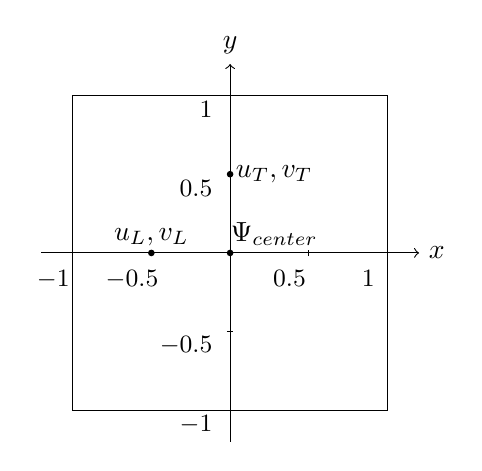
\begin{tikzpicture}[scale=2]

  \draw (-1,-1) rectangle (1,1);
  \draw (-1,-1) rectangle (1,1);

  \draw[->] (-1.2,0) -- (1.2,0) node[right] {$x$};
  \foreach \x in {-1,-0.5,0.5,1}
      \draw (\x,-0.02) -- (\x,0.02) node[right=-7pt, below=4pt] {\small $\x$};
  
  \draw[->] (0,-1.2) -- (0,1.2) node[above] {$y$};
  \foreach \y in {-1,-0.5,0.5,1}
    \draw (-0.02,\y) -- (0.02,\y) node[below=5pt, left=4pt] {\small $\y$};

  \node at (0.28,0.5) {$u_T, v_T$};
  \fill (0, 0.5) circle [radius=0.6pt];

  \node at (-0.5,0.1) {$u_L, v_L$};
  \fill (-0.5,0) circle [radius=0.6pt];

  \node at (0.28,0.12) {$\Psi_{center}$};
  \fill (0,0) circle [radius=0.6pt];
\end{tikzpicture}
\caption{Square domain $(x,y) \in [-1,1]\times[-1,1]$ for the four-sided cavity.}
\label{fig:cav_domain}
\end{figure}

As shown in figure \ref{fig:cav_4s} of the four-sided cavity flow, all lids
have the same tangential velocity. The original discontinuous boundary
conditions are,

\begin{align}
u(x,\pm 1,t) &= \pm 1,\label{non_reg_u_bca} \\
v(x,\pm 1,t) &= 0, \\
u(\pm 1,y,t) &= 0, \\
v(\pm 1,y,t) &= \pm 1.\label{non_reg_u_bcb}
\end{align}

To discretize \eqref{eq:str} using a spectral method, \eqref{non_reg_u_bca} and
\eqref{non_reg_u_bcb} are replaced by the regularized boundary conditions,
which impose a zero velocity at all four corners of the cavity,
\begin{align}
u(x,\pm 1,t) &= \pm\left[\left(\rme^{k_0(x - 1)} - 1\right)
  \left(\rme^{-k_0(x + 1)} - 1\right)\right]^2, \label{reg_u_bca} \\
v(\pm 1,y,t) &= \pm\left[\left(\rme^{k_0(y - 1)} - 1\right)
  \left(\rme^{-k_0(y + 1)} - 1\right)\right]^2. \label{reg_u_bcb}
\end{align}

The exponential regularization function is adapted from \citet{lopez2017}.
Where $k_0$ is a suitable parameter controlling the slope of the decay of the
velocity profile near the corners. In this study, we set $k_0=10$ to get a
suitable but not too extreme decay for the velocity at the edges. Figure
\ref{bc_profile} shows such a profile.

\begin{figure}[ht]
\center
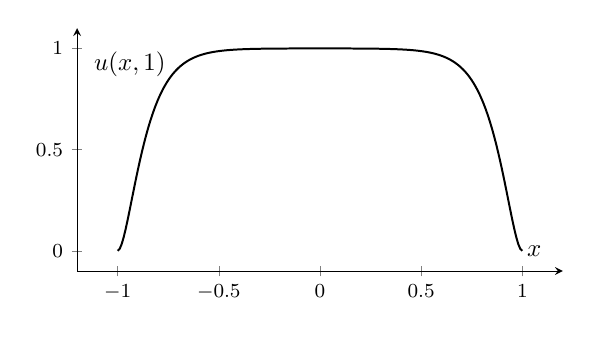
\begin{tikzpicture}[scale=0.9]
  \begin{axis}[
    xlabel={$x$},
    ylabel={$u(x, 1)$},
    xlabel style={at={(current axis.right of origin)}, anchor=west}, 
    ylabel style={at={(0.2,0.85)}, anchor=east, rotate=-90},
    domain=-1.0:1.0,
    samples=200,
    axis lines=left,
    xmin=-1.0, xmax=1.0,
    ymin=0.0, ymax=1.0,
    ticklabel style={font=\footnotesize},
    enlargelimits=true,
    axis equal image
  ]
    \addplot[black, thick] {((exp(10*(x-1))-1)*(exp(-10*(x+1))-1))^2};
  \end{axis}
\end{tikzpicture}
\caption{\label{bc_profile} Regularized horizontal velocity profile
  \eqref{reg_u_bca} at the top wall $y=1$ for $k_0=10$.}
\end{figure}

In order to compare the results of this work with the previous literature, the
Reynolds number has to be scaled. The $[0,1] \times [0,1]$ domain used in
\citet{wahba2009} and the subsequent studies mean that reference length
$l_{ref}$ used is, therefore, half the length $l$ used here. Thus the relation
of the Reynolds numbers is,
\vspace{-8pt}
\begin{align}
\Rey = \frac{U \cdot l}{\nu} 
  = \frac{sU_{ref} \cdot 2l_{ref}}{\nu} = 2s \cdot \Rey_{ref}.
\end{align}

This implies a scaling factor of $s=\frac{1}{2}$, and the Reynolds number of
previous studies has to be divided by $2$. In all further comparisons of
results, the reference Reynolds numbers will be scaled to the presented
symmetrical domain.

\subsection{A Physical or Mathematical Problem?}

The final important point to make is that the 2D problem must be studied
cautiously. The paper of \cite{eturk2009} concludes that the single lid-driven
cavity represents \emph{fictitious} flow at high Reynolds numbers. Fictitious
meaning that the problem from a physical point of view would no longer be
purely 2D because instabilities in the third dimension would influence the
flow. However, numerical solutions exist at high Reynolds numbers for the
two-dimensional case.

Furthermore, it is hard to replicate the lid-driven cavity experimentally with
regularized boundary conditions. This problem gets even worse considering the
four-sided cavity flow and the different velocity directions at all lids.

Using a regularized version, as presented above, will help to obtain numerical
accurate results, but it makes it even harder to reproduce in practice. From
the point of view of a benchmark for an instability analysis for different
solvers, the resulting flow (whether fictional or not) should at least be
precisely computable. This report will focus on this main aspect, that is the
accurate computation of a well-posed mathematical problem. 
